% Drawing 146/03-2 -- folder 146, batch 03, archive page 57 (PDF page 58).
% Transcription: en haut à gauche, une sphère portant un grand cercle (équateur) avec quatre petits cercles pointés ; légende « 4 sommets, deux faces ». Une flèche « deux façons » mène à une seconde sphère, même équateur à quatre sommets cerclés, coupé par un grand cercle méridien (« cercle marqué ») ; légende « 1 cercle marqué, 6 sommets, 4 faces ».
% Kind: cell decomposition of the sphere. Method 3 (encoded, rendered from the data). Status: ok.
% Notes: Two spheres: equator with four ringed vertices; then the same cut by a marked great circle (meridian). Encoded as cellular/1; his counts (4 sommets, deux faces; 6 sommets, 4 faces) are reproduced. The legends under the figures (« 3 possibilités pour I », « 6 possibilités pour I ») are text of the transcription and are not redrawn.
% Coordinates: 1 unit = 1 mm = 1/100 of the crop width (bbox in page fractions: [0.13, 0.11, 0.85, 0.33]).
% Redrawn by Claude (claude-opus-5-5), issue #73 pilot, 2026-11-07; not checked by a human; not compiled (no TeX in the session).
% Rights: reproduces part of the work -- behind RENDER_TRANSCRIPTS, never published by itself.
\documentclass[tikz,border=3pt]{standalone}
\usepackage{amsmath,amssymb}
\usetikzlibrary{patterns,arrows.meta}
\tikzset{pencil/.style={black!45}, struck/.style={black!35}, mark/.style={circle,draw,inner sep=1.3pt}, pt/.style={circle,fill,inner sep=0.9pt}, opt/.style={circle,draw,fill=white,inner sep=1.1pt}}
\begin{document}
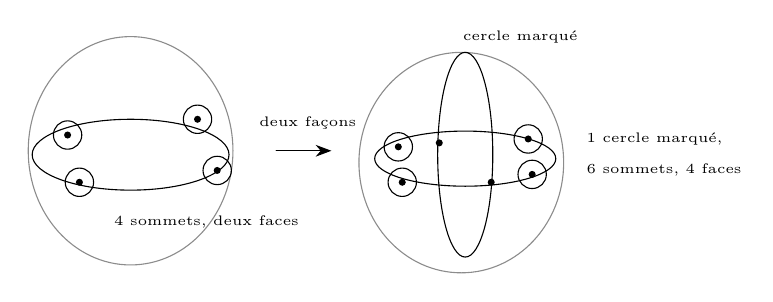
\begin{tikzpicture}[x=1mm,y=1mm,line cap=round,line join=round,font=\scriptsize]
\draw[pencil] (22.5,-18.5) ellipse[x radius=13, y radius=14.5];
\draw (22.5,-19) ellipse[x radius=12.5, y radius=4.5];
\draw (14.5,-16.5) circle[radius=1.8];
\draw (16,-22.5) circle[radius=1.8];
\draw (31,-14.5) circle[radius=1.8];
\draw (33.5,-21) circle[radius=1.8];
\node[pt] at (14.5,-16.5) {};
\node[pt] at (16,-22.5) {};
\node[pt] at (31,-14.5) {};
\node[pt] at (33.5,-21) {};
\draw[-{Stealth[length=2mm]}] (41,-18.5) -- (48,-18.5);
\node[inner sep=1pt] at (45,-15) {\tiny deux façons};
\node[inner sep=1pt,anchor=west] at (20,-27.5) {\tiny 4 sommets, deux faces};
\draw[pencil] (64.5,-20) ellipse[x radius=13, y radius=14];
\draw (65,-19.5) ellipse[x radius=11.5, y radius=3.5];
\draw (65,-19) ellipse[x radius=3.5, y radius=13];
\draw (56.5,-18) circle[radius=1.8];
\draw (57,-22.5) circle[radius=1.8];
\draw (73,-17) circle[radius=1.8];
\draw (73.5,-21.5) circle[radius=1.8];
\node[pt] at (56.5,-18) {};
\node[pt] at (57,-22.5) {};
\node[pt] at (73,-17) {};
\node[pt] at (73.5,-21.5) {};
\node[pt] at (61.7,-17.5) {};
\node[pt] at (68.3,-22.5) {};
\node[inner sep=1pt] at (72,-4) {\tiny cercle marqué};
\node[inner sep=1pt,anchor=west] at (80,-17) {\tiny 1 cercle marqué,};
\node[inner sep=1pt,anchor=west] at (80,-21) {\tiny 6 sommets, 4 faces};
\end{tikzpicture}
\end{document}
